% ======================================================================
% Endterm-Cheatsheet WS 24/25.
% ======================================================================
\documentclass[threecolumn, 5pt, german]{latex4ei/latex4ei_sheet}

%Matlab settings
\lstset{language=Matlab, basicstyle=\normalsize\ttfamily}

%Custom packages
\usepackage{tikz}

\title{Matlab-Cheatsheet für Signaltheorie}
\author{Roman Eisenlauer}
\myemail{roman.eisenlauer@tum.de}
\mywebsite{www.latex4ei.de}

\begin{document}
	\maketitle
	
	% ======================================================================
	% SECTION 1: GRUNDLAGEN
	% ======================================================================
	\section{Grundlagen}
	
	% ----------------------------------------------------------------------
	\begin{sectionbox}
	
		\subsection{Erstellung von Vektoren}
		
		\subsubsection{Zeilenvektor-Erstellung}
		
		\begin{lstlisting}
% Zeilenvektor mit Startwert A, Endwert B und Schritten von 1:
x = A:B

% Zeilenvektor mit Startwert A, Endwert B und Schritten von C:
x = A:C:B
		\end{lstlisting}
		
		\subsubsection{Zeitvektor-Erstellung}
		
		\begin{lstlisting}
% Zeitvektor mit Startwert 0s, Abtastrate fs (in Samples / s)
% und Zeitdauer T (in s):
t = 0:1/fs:T-1/fs;

% oder
N = fs * T  % Sample-Anzahl
t = (0:N-1)/fs;
		\end{lstlisting}
	\end{sectionbox}
	
	% ----------------------------------------------------------------------
	\begin{sectionbox}
	
		\subsection{Standard-Signale}
		
		\subsubsection{Sinus- und Kosinus-Signale}
		
		\begin{lstlisting}
% Sinus-Signal mit Frequenz f (in Hz) ueber Zeitvektor t (in s):
x = sin(2*pi*f*t) % Kosinus: cos(..)
		\end{lstlisting}
		
		\subsubsection{Rechtecksignal}
		
		\begin{lstlisting}
% Rechtecksignal von 0.5s Laenge, startet bei 0.3s
% mit logischer Indizierung!
T = 1;                  % Zeitdauer in s
fs = 10;                % Abtastrate in Samples / s
t = 0:1/fs:1-1/fs;      % Zeitvektor in s (dt = 1/fs)
x = zeros(size(t));     % Initialisierung mit 0en
x(t>=0.3 & t<0.8)=1.0;   % 1er an richtigen Stellen setzen
		\end{lstlisting}
		
		\subsubsection{Sprungfunktion und weitere Funktionen}
		
		\begin{lstlisting}
% Sprungfunktion u(t) (=1 fuer t>=0) ueber Zeitvektor t
u = heaviside(t)

exp(t)       % Exponentialfunktion
sqrt(t)      % Quadratwurzel
log(t)       % Natuerlicher Logarithmus
t.^2;        % Parabel
		\end{lstlisting}
	\end{sectionbox}
	
	% ----------------------------------------------------------------------
	% --- Signal-Operationen in mehrere Blöcke aufgeteilt ---
	
	\begin{sectionbox}
	
		\subsection{Signal-Operationen}
		
		\subsubsection{Differentiation}
		
		\begin{lstlisting}
% Ableiten (skaliert) Vektorlaenge reduziert sich um 1!
x_D = diff(x)/dt;
		\end{lstlisting}

		\subsubsection{Integration}
		
		\begin{lstlisting}
% Integrieren (skaliert)
% 1. Stammfunktion (Ergebnis ist ein Vektor)
x_I = cumsum(x)*dt;
% 2. Bestimmtes Integral, Flaeche (Ergebnis ist eine Zahl)
I = sum(x)*dt;
		\end{lstlisting}

		\subsubsection{Arithmetische Operationen}
		
		\begin{lstlisting}
x_ = x + A;   % Konstante A aufaddieren
x_ = x * A;   % Konstante A heranmultiplizieren
y = x1 + x2;  % Element-weise Addition
y = x1 .* x2; % Element-weise Multiplikation
y = x1./x2;   % Element-weise Division
y = x.^2;     % Element-weise Quadrierung
		\end{lstlisting}

		\subsubsection{Diskrete Faltung und Padding}
		
		\begin{lstlisting}
% Diskrete Faltung
y = conv(x,h); % length(y)=length(x)+length(h)-1;

% Signal mit anhaengenden 0en auffuellen (Anzahl: N0)
% x muss ein Zeilenvektor sein!
x_ = [x, zeros(1,N0)];
		\end{lstlisting}

		\subsubsection{Betrag und Real-/Imaginärteil}
		\begin{lstlisting}
y = abs(x);   % Betrag
y = real(x);  % Realteil
y = imag(x);  % Imaginaerteil
		\end{lstlisting}
	\end{sectionbox}
	
	% ----------------------------------------------------------------------
	\begin{sectionbox}
	
		\subsection{Indizierung}
		
		\subsubsection{Einzelne und mehrere Elemente}
		
		\begin{lstlisting}
x = [0,2,4,6,8,10,12,14,16,18];

% Einzelner Wert
x_1 = x(1); % x_1 = 0

% Mehrere Werte (erstes, viertes und 7tes Element)
x_i = x([1,4,7]); % x_i = [0,6,12]

% Bereich (4tes bis einschl. 8tes Elemet)
x_i = x(4:8);  % x_i = [6,8,10,12,14]
		\end{lstlisting}

		\subsubsection{Logische Indizierung}
		\begin{lstlisting}
% Logische Indizierung:
x_neu = x(x>10); % x_neu = [12,14,16,18];

% Anwendung auf einen anderen Vektor (z.B. Zeitvektor)
t = 0:9; % [0,1,2,3,4,5,6,7,8,9]

% Alle Zeitwerte fuer die gilt x>10
t_neu = t(x>10); % t_neu = [6,7,8,9]

% alle x-Werte fuer die gilt t>5
x_neu_2 = x(t>5); % x_neu_2 = [12,14,16,18];

% Zusammengesetzte logische Ausdruecke
x_neu_3 = x(t>=2 & t<8); % x_neu_3 = [4,6,8,10,12,14]
		\end{lstlisting}
	\end{sectionbox}
	
	% ----------------------------------------------------------------------
	\begin{sectionbox}
	
		\subsection{Elemente finden}
		
		\subsubsection{Maximum und Minimum}
		
		\begin{lstlisting}
% Irgendein Signal x
x = [1,-4,-3,3,-2,2];

% Maximalwert
x_max = max(x) % x_max = 3
% Maximalwert und zugehoeriger Index
[x_max, i_max] = max(x) % x_max = 3, i_max = 4

% Minimalwert
x_min = min(x) % x_min = -4
% Minimalwert und zugehoeriger Index
[x_min, i_min] = min(x) % x_min = -4, i_min = 2
		\end{lstlisting}

		\subsubsection{Suche nach Elementen und Indizes}
		
		\begin{lstlisting}
% Wo ist x gleich 3 ?
i_3 = find(x==3); % i_3 = 4;

% Wo ist x am naechsten an 2.23?
[abs_err,i_] = min(abs(x-2.23)); % i_ = 6, (abs_err = 0.23)
% abs_err will ich nicht wissen: Platzhalter ~
[~,i_] = min(abs(x-2.23)); % i_ = 6

% Auswertung von x bei t=2
t = 0:5; % Zeitvektor (fs=1)
x_t2 = x(t==2); % x_t2 = -3
		\end{lstlisting}
	\end{sectionbox}
	
	% ----------------------------------------------------------------------
	\begin{sectionbox}
	
		\subsection{Funktions-Definitionen für Vektoren}
		
		\subsubsection{Definition von Funktionen}
		
		\begin{lstlisting}
% Definition eines Zeitsignals als Funktion
x_fun = @(t) exp(-t);

% Definition von t
T_start = -2;    % Startzeitpunkt in s
T_stop = 5;      % Endzeitpunkt in s
fs = 100;        % Abtastrate in Samples/s
t = T_start:1/fs:T_stop-1/fs;

% Auswertung:
x = x_fun(t);
		\end{lstlisting}

		\subsubsection{Bereichsweise Definition und Transformation}
		
		\begin{lstlisting}
% Bereichsweise definition (aus Uebung 4, Aufgabe 1c)
x3_fun = @(t) (t>=-1 & t<0) .* (t+1) + (t>=0 & t<1) .* (1-t)

% Signaltransformation durch einfaches Einsetzen:
% x4(t) = x3(t) + 2 * x3(1/2*t -1)
x4 = x3_fun(t) + 2 * x3_fun(1/2*t-1)
		\end{lstlisting}
		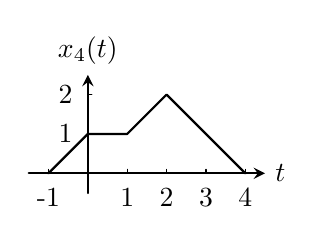
\begin{tikzpicture}[>=stealth, line cap=round, line join=round, scale=0.5]

  % Achsen zeichnen
  \draw[->,thick] (-1.5,0) -- (4.5,0) node[right] {$t$};
  \draw[->,thick] (0,-0.5) -- (0,2.5) node[above] {$x_4(t)$};

  % Ticks auf der x-Achse
  \foreach \x in {-1, ,1,2,3,4} {
    \draw (\x,0) -- (\x,0.1);          % kleiner Strich am Tick
    \node[below=2pt] at (\x,0) {\x};   % Tick-Beschriftung
  }

  % Ticks auf der y-Achse
  \foreach \y in {1,2} {
    \draw (0,\y) -- (0.1,\y);
    \node[left=2pt] at (0,\y) {\y};
  }

  % Das stückweise definierte Signal:
  % von t=-1 bis 0: x4(t) = t+1
  % von t=0 bis 1:  x4(t) = 1
  % von t=1 bis 2:  x4(t) = t
  % von t=2 bis 4:  x4(t) = -t + 4
  \draw[thick] 
    (-1,0) -- (0,1)  % t=-1..0
    -- (1,1)         % t=0..1
    -- (2,2)         % t=1..2
    -- (4,0);        % t=2..4

  % Optional: Titel oder Funktionslabel an passender Stelle
  % \node at (2,2.2) {$x_4(t)$};

		\end{tikzpicture}
	\end{sectionbox}
	
	% ======================================================================
	% SECTION 2: DFT/FFT
	% ======================================================================
	\section{DFT/FFT}
	
	\begin{sectionbox}
	
		\subsection{Realisierung der DFT des Signalvektors x}
		
		\begin{lstlisting}
X = fft(x) 
		\end{lstlisting}
	\end{sectionbox}
	
	\begin{sectionbox}
	
		\subsection{Skalierung zur komplexen Fourier-Reihe / zweiseitiges Amplitudenspektrum}
		
		\subsubsection{Berechnung der Fourierkoeffizienten}
		
		\begin{lstlisting}
X = fft(x) / N;

% Fourierkoeffizienten fuer +k und -k
% c_{k} = X[k]
cpk = X(k+1);  % Indizierung bei Matlab startet bei 1

% c_{-k} = X[N-k]
cmk = X(N-k+1) % Indizierung bei Matlab startet bei 1
		\end{lstlisting}

		\subsubsection{Frequenzachse und Umordnung}
		
		\begin{lstlisting}
% Frequenzachse
df = fs / N;              % Frequenzaufloesung
f = 0:df:fs-df;           % Positiver Frequenzvektor
f(f>=fs/2) = f(f>=fs/2) - fs; % Ab fs/2 -> fs abziehen!

% Umdrehen: Zweiseitiges Amplitudenspektrum
X_ds = fftshift(X);
f = fftshift(f);
		\end{lstlisting}
	\end{sectionbox}
	
	\begin{sectionbox}
	
		\subsection{Einseitiges Amplitudenspektrum}
		
		\subsubsection{Berechnung und Anpassung}
		
		\begin{lstlisting}
X = abs(fft(x)) / N;  
X = X(1:floor(N/2+1)); % Positive Achse. (bei geradem N: fs/2 inklusive)
X_ss = X;

% N ist gerade:
X_ss(2:end-1) = X_ss(2:end-1) * 2;

% ODER: N ist ungerade:
X_ss(2:end) = X_ss(2:end) * 2;
		\end{lstlisting}

		\subsubsection{Frequenzvektor}
		\begin{lstlisting}
df = fs / N;
f = 0:df:floor(N/2)*df;  % Positiver Frequenzvektor
		\end{lstlisting}
	\end{sectionbox}
	
	% ======================================================================
	% SECTION 3: PLOTTEN
	% ======================================================================
	\section{Plotten}
	
	\begin{sectionbox}
	
		\subsection{Erstellen von Plot-Fenstern}
		
		\begin{lstlisting}
figure;                   % Erstellen einer figure
		\end{lstlisting}
	\end{sectionbox}
	
	\begin{sectionbox}
	
		\subsection{Plot-Befehle}
		
		\begin{lstlisting}
plot(t,x)                 % Signal x ueber t plotten
plot(t,x,"LineWidth",1.5) % mit definierter Linienstaerke
plot(t,x,"LineStyle","--")% mit alternativem Linienstil
semilogx(t,x)             % X-Achse logarithmisch
semilogy(t,x)             % Y-Achse logarithmisch
loglog(t,x)               % Doppelt-logarithmische Darstellung
		\end{lstlisting}
	\end{sectionbox}
	
	\begin{sectionbox}
	
		\subsection{Plot-Optionen}
		
		\begin{lstlisting}
% Stelle alle weiteren Plots im gleichen Fenster dar
hold on
% Stelle weitere Plots nicht im gleichen Fenster dar
hold off
		\end{lstlisting}
	\end{sectionbox}
	
	\begin{sectionbox}
	
		\subsection{Achsenbeschriftung und Legenden}
		
		\begin{lstlisting}
legend(["x1(t)","x2(t)"]) % Legende (in diesem Fall 2 Eintraege)
xlabel("t in s")          % X-Achsenbeschriftung
ylabel("Amplitude in V")  % Y-Achsenbeschriftung
xlim([a,b]);              % X-Achsenlimits
ylim([a,b]);              % Y-Achsenlimits
xticks([0.1,0.3,1.0])     % Ticks auf X-Achse manuell setzen
yticks([0.1,0.3,1.0])     % Ticks auf Y-Achse manuell setzen
		\end{lstlisting}
	\end{sectionbox}
	
	\begin{sectionbox}
	
		\subsection{Tick-Anpassungen}
		
		\begin{lstlisting}
% Labels fuer Ticks auf X-Achse manuell setzen
xticklabels(["0.1","0.3","1.0"])
% Labels fuer Ticks auf Y-Achse manuell setzen
yticklabels(["0.1","0.3","1.0"])
		\end{lstlisting}
	\end{sectionbox}
	
	\begin{sectionbox}
	
		\subsection{Anpassung der Figure-Größe}
		
		\begin{lstlisting}
% "Insider-Tipp": Groesse der figure auf definiertes Format in cm skalieren:
set(gcf, 'Units', 'Centimeters', 'Position', [0 0 8.4 9], ...
'PaperPositionMode', 'auto')
		\end{lstlisting}
	\end{sectionbox}
	
\end{document}
